
\section*{Extra Slides}

\begin{frame}
  \sectionpage
\end{frame}

\begin{frame}{Results}
  \begin{table}
    \centering
    \caption{
      \emph{Effect of different attack configurations (untargeted) on all baselines.}
      \texttt{RA} is RADAR, \texttt{FG} is \texttt{FoolsGold}, \texttt{FA} is \texttt{FedAvg} (on \emph{all} participants), and \texttt{FC} is \texttt{FedAvg} ideally clustered per dataset.
    }

    \footnotesize

    \newcommand{\hl}{}
    \only<2>{\renewcommand{\hl}{\cellcolor{imta-green!30}}}


  
    \setlength\tabcolsep{1ex}
    \begin{tabularx}{.8\textwidth}{lX|rrrr|rrrr}
      \toprule % ---------------------------------
      \multicolumn{2}{c|}{\multirow{2}{*}{\textbf{Scenario}}} & \multicolumn{4}{c|}{\textbf{Mean accuracy} (\%)} & \multicolumn{4}{c}{\textbf{\gls{asr}} (\%)} \\
      & & \multicolumn{1}{c}{\texttt{RA}} & \multicolumn{1}{c}{\texttt{FG}} & \multicolumn{1}{c}{\texttt{FA}} & \multicolumn{1}{c|}{\texttt{FC}} & \multicolumn{1}{c}{\texttt{RA}} & \multicolumn{1}{c}{\texttt{FG}} & \multicolumn{1}{c}{\texttt{FA}} & \multicolumn{1}{c}{\texttt{FC}} \\
      \midrule % ---------------------------------
      % TARGETED ATTACKS
      \multicolumn{2}{l|}{\textbf{Targeted} (\texttt{100T})} & & & & & & & & \\
                  & \texttt{Benign}       & \hl 99.07 & 55.04 & 79.49 & \textbf{99.24} & \hl \textbf{0.00} &  5.17 & 5.10 &  0.09 \\
                  & \texttt{Lone}         & \hl 99.06 & 60.51 & 77.38 & \textbf{99.22} & \hl \textbf{0.00} & 93.82 & 6.73 &  0.45 \\
                  & \texttt{Collud. min.} & \hl \textbf{98.96} & 54.64 & 78.48 & 98.33 & \hl \textbf{0.00} &  2.97 & 9.99 & 53.40 \\
                  & \texttt{Collud. maj.} & \hl \textbf{98.28} & 85.10 & 79.40 & 98.22 & \hl \only<3>{\bfseries\color{red}} 73.39 & \textbf{8.10} & 17.65 & 59.36 \\
      \midrule % ---------------------------------
      % UNTARGETED ATTACKS
      \multicolumn{2}{l|}{\textbf{Untargeted} (\texttt{100U})} & & & & & & & & \\
      & \texttt{Benign}        & \hl 99.07 & 55.04 & 79.49 & \textbf{99.24} & \hl 0.09  & 0.39 & 33.30 & \textbf{0.06} \\
      & \texttt{Lone}          & \hl 98.96 & 49.56 & 78.38 & \textbf{99.22} &\hl \textbf{0.08} & 99.89 & 54.70 & 0.12 \\
      & \texttt{Collud. min.}  & \hl \textbf{98.98} & 49.67 & 72.47 & 97.69 & \hl 0.10 & \textbf{0.04} & 44.53 & 6.26 \\
      & \texttt{Collud. maj.}  & \hl \textbf{98.96} & 69.09 & 81.87 & 75.66 & \hl \textbf{0.08} & 38.98 & 59.49 & 94.36 \\          
      \bottomrule % ---------------------------------
      \small & \multicolumn{1}{c}{} & \multicolumn{4}{c}{\emph{higher is better}} & \multicolumn{4}{c}{\emph{lower is better}}
    \end{tabularx}
  \end{table}
  
\end{frame}

\begin{frame}{Results}
  \begin{table}
    \centering
    \caption{
      \emph{Effect of different attack configurations (untargeted) on all baselines.}
      \texttt{RA} is RADAR, \texttt{FG} is \texttt{FoolsGold}, \texttt{FA} is \texttt{FedAvg} (on \emph{all} participants), and \texttt{FC} is \texttt{FedAvg} ideally clustered per dataset.
    }

    \footnotesize

    \newcommand{\hl}{}
    \only<2>{\renewcommand{\hl}{\cellcolor{imta-green!30}}}


  
    \setlength\tabcolsep{1ex}
    \begin{tabularx}{.8\textwidth}{lX|rrrr|rrrr}
      \toprule % ---------------------------------
      \multicolumn{2}{c|}{\multirow{2}{*}{\textbf{Scenario}}} & \multicolumn{4}{c|}{\textbf{Mean accuracy} (\%)} & \multicolumn{4}{c}{\textbf{\gls{asr}} (\%)} \\
      & & \multicolumn{1}{c}{\texttt{RA}} & \multicolumn{1}{c}{\texttt{FG}} & \multicolumn{1}{c}{\texttt{FA}} & \multicolumn{1}{c|}{\texttt{FC}} & \multicolumn{1}{c}{\texttt{RA}} & \multicolumn{1}{c}{\texttt{FG}} & \multicolumn{1}{c}{\texttt{FA}} & \multicolumn{1}{c}{\texttt{FC}} \\
      \midrule % ---------------------------------
      % TARGETED ATTACKS
      \multicolumn{2}{l|}{\textbf{Targeted} (\texttt{100T})} & & & & & & & & \\
                  & \texttt{Benign}       & \hl 99.07 & 55.04 & 79.49 & \textbf{99.24} & \hl \textbf{0.00} &  5.17 & 5.10 &  0.09 \\
                  & \texttt{Lone}         & \hl 99.06 & 60.51 & 77.38 & \textbf{99.22} & \hl \textbf{0.00} & 93.82 & 6.73 &  0.45 \\
                  & \texttt{Collud. min.} & \hl \textbf{98.96} & 54.64 & 78.48 & 98.33 & \hl \textbf{0.00} &  2.97 & 9.99 & 53.40 \\
                  & \texttt{Collud. maj.} & \hl \textbf{98.28} & 85.10 & 79.40 & 98.22 & \hl \only<3>{\bfseries\color{red}} 73.39 & \textbf{8.10} & 17.65 & 59.36 \\
      \midrule % ---------------------------------
      % UNTARGETED ATTACKS
      \multicolumn{2}{l|}{\textbf{Untargeted} (\texttt{100U})} & & & & & & & & \\
      & \texttt{Benign}        & \hl 99.07 & 55.04 & 79.49 & \textbf{99.24} & \hl 0.09  & 0.39 & 33.30 & \textbf{0.06} \\
      & \texttt{Lone}          & \hl 98.96 & 49.56 & 78.38 & \textbf{99.22} &\hl \textbf{0.08} & 99.89 & 54.70 & 0.12 \\
      & \texttt{Collud. min.}  & \hl \textbf{98.98} & 49.67 & 72.47 & 97.69 & \hl 0.10 & \textbf{0.04} & 44.53 & 6.26 \\
      & \texttt{Collud. maj.}  & \hl \textbf{98.96} & 69.09 & 81.87 & 75.66 & \hl \textbf{0.08} & 38.98 & 59.49 & 94.36 \\          
      \bottomrule % ---------------------------------
      \small & \multicolumn{1}{c}{} & \multicolumn{4}{c}{\emph{higher is better}} & \multicolumn{4}{c}{\emph{lower is better}}
    \end{tabularx}
  \end{table}
  
\end{frame}
\begin{frame}{Intrusion Detection}
  
  \textbf{Machine Learning (ML) for Network-based Intrusion Detection Systems (NIDSs)}
  \begin{itemize}
    \item Detect \alert{malicious} activities (\ie, \textit{misuse detection}) or \alert{anomalies} (\ie, \textit{anomaly detection}).
    \item Various types of algorithms: \alert<2>{supervised}, unsupervised, semi-supervised, reinforcement learning, \textit{etc}.
    \item Great performance with Deep Learning (DL) (on public datasets at least).
  \end{itemize}
  \bigskip
    
  \begin{figure}
    \centering
    \makebox[\textwidth][c]{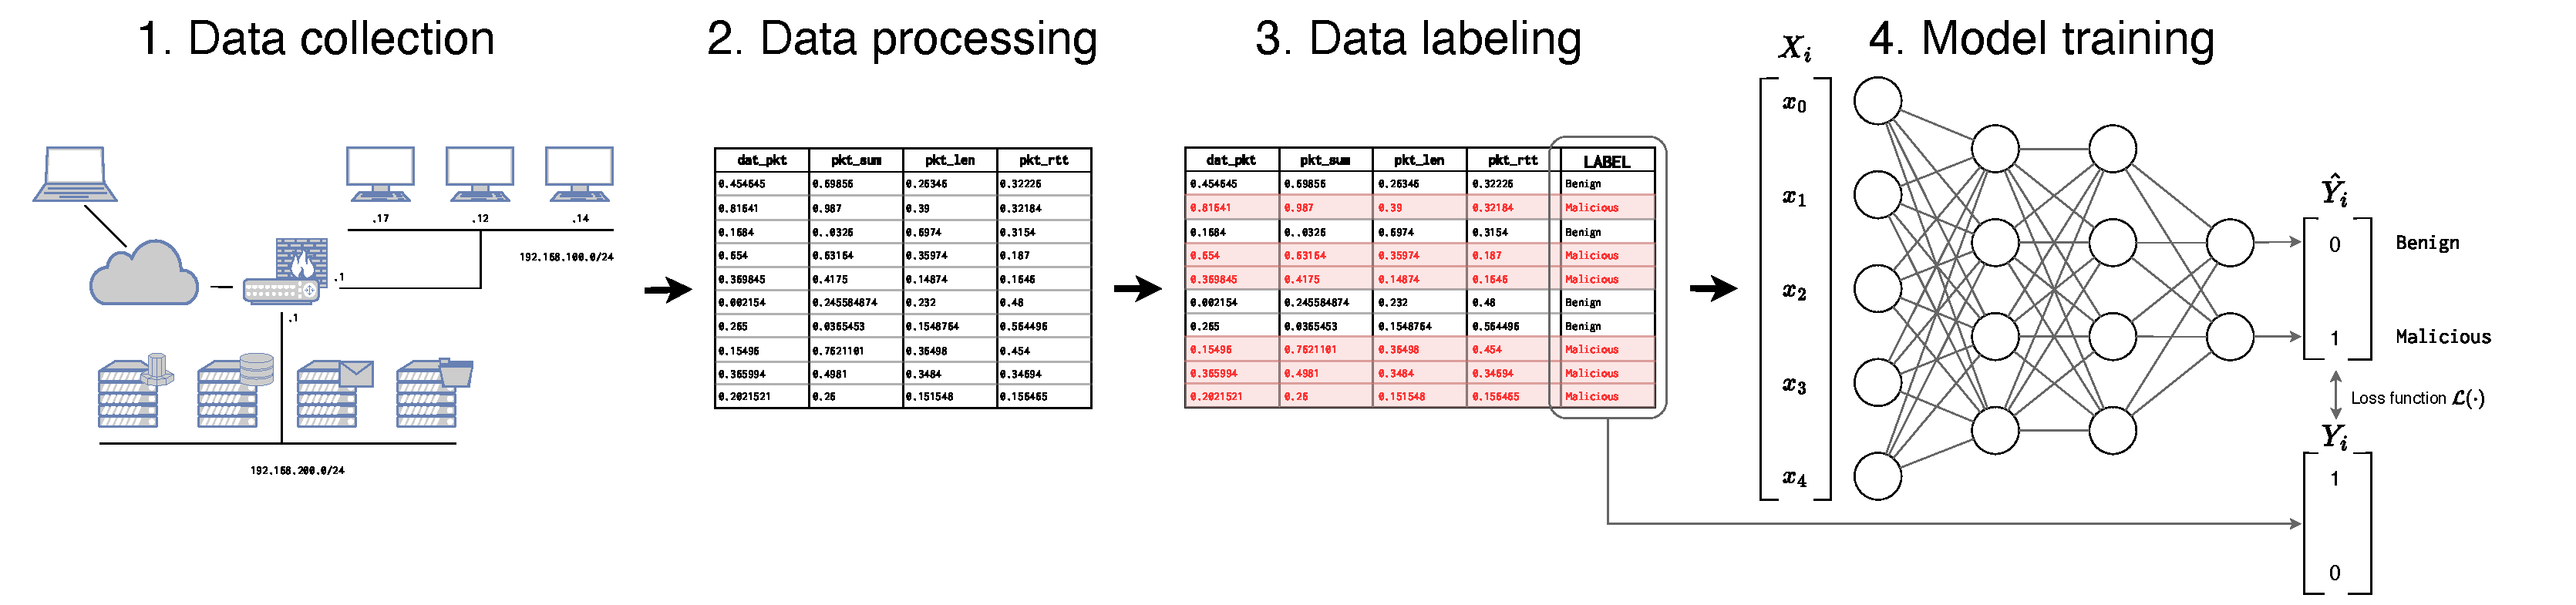
\includegraphics[width=.9\textwidth]{figures/intro/mlp-workflow.pdf}}
    \caption{Typical workflow for ML-based NIDSs.}
  \end{figure}
\end{frame}

\begin{frame}{Intrusion Detection}

  \begin{columns}
    \begin{column}{0.5\textwidth}
        \textbf{Challenges:}
        \begin{itemize}
          \item not enough labelled data;
          \item risk of local bias or skewed data distribution;
          \item inefficient against new attacks, especially \alert{supervised} approaches.
        \end{itemize}
    \end{column}

    \begin{column}{0.5\textwidth}
      \begin{figure}
        \centering
        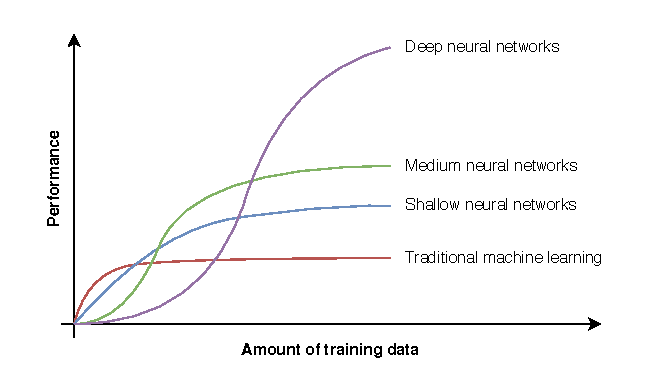
\includegraphics[width=\linewidth]{figures/intro/ml-perf}
      \end{figure}
    \end{column}
  \end{columns}
\end{frame}

\begin{frame}{Scaling Intrusion Detection}

  \textbf{Federated Learning (FL)}
  
  \begin{itemize}
    \item Novel-\emph{ish} distributed ML paradigm (Google, 2017)~\cite{mcmahan_Communicationefficientlearningdeep_2017}.
    \item Distributed clients can train a common model without sharing their training data.
    \item Privacy-preserving: high level of abstraction for the shared models preventing data leakage.
  \end{itemize}
\end{frame}

\begin{frame}{FL Fundamentals}
  \vspace{-1em}
  \begin{figure}
    \centering
    \only<1>{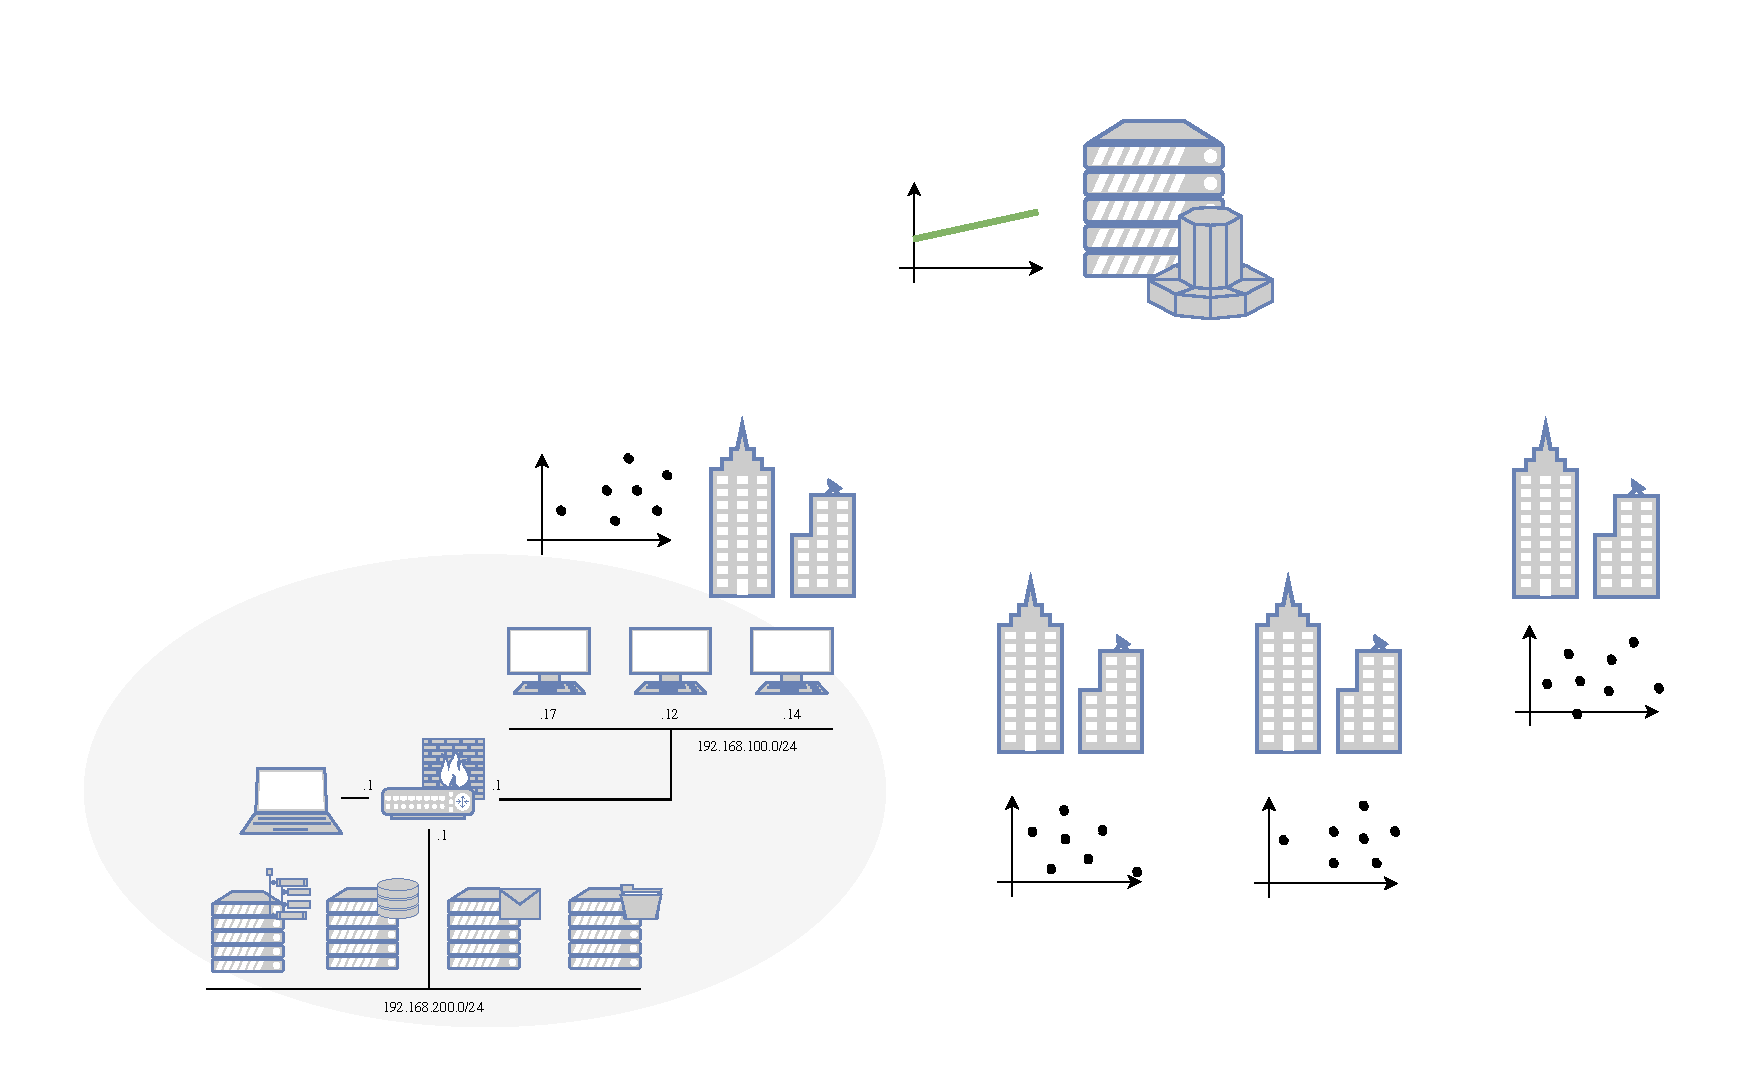
\includegraphics[width=.75\linewidth]{./figures/intro/fl/0.pdf}}%
    \only<2>{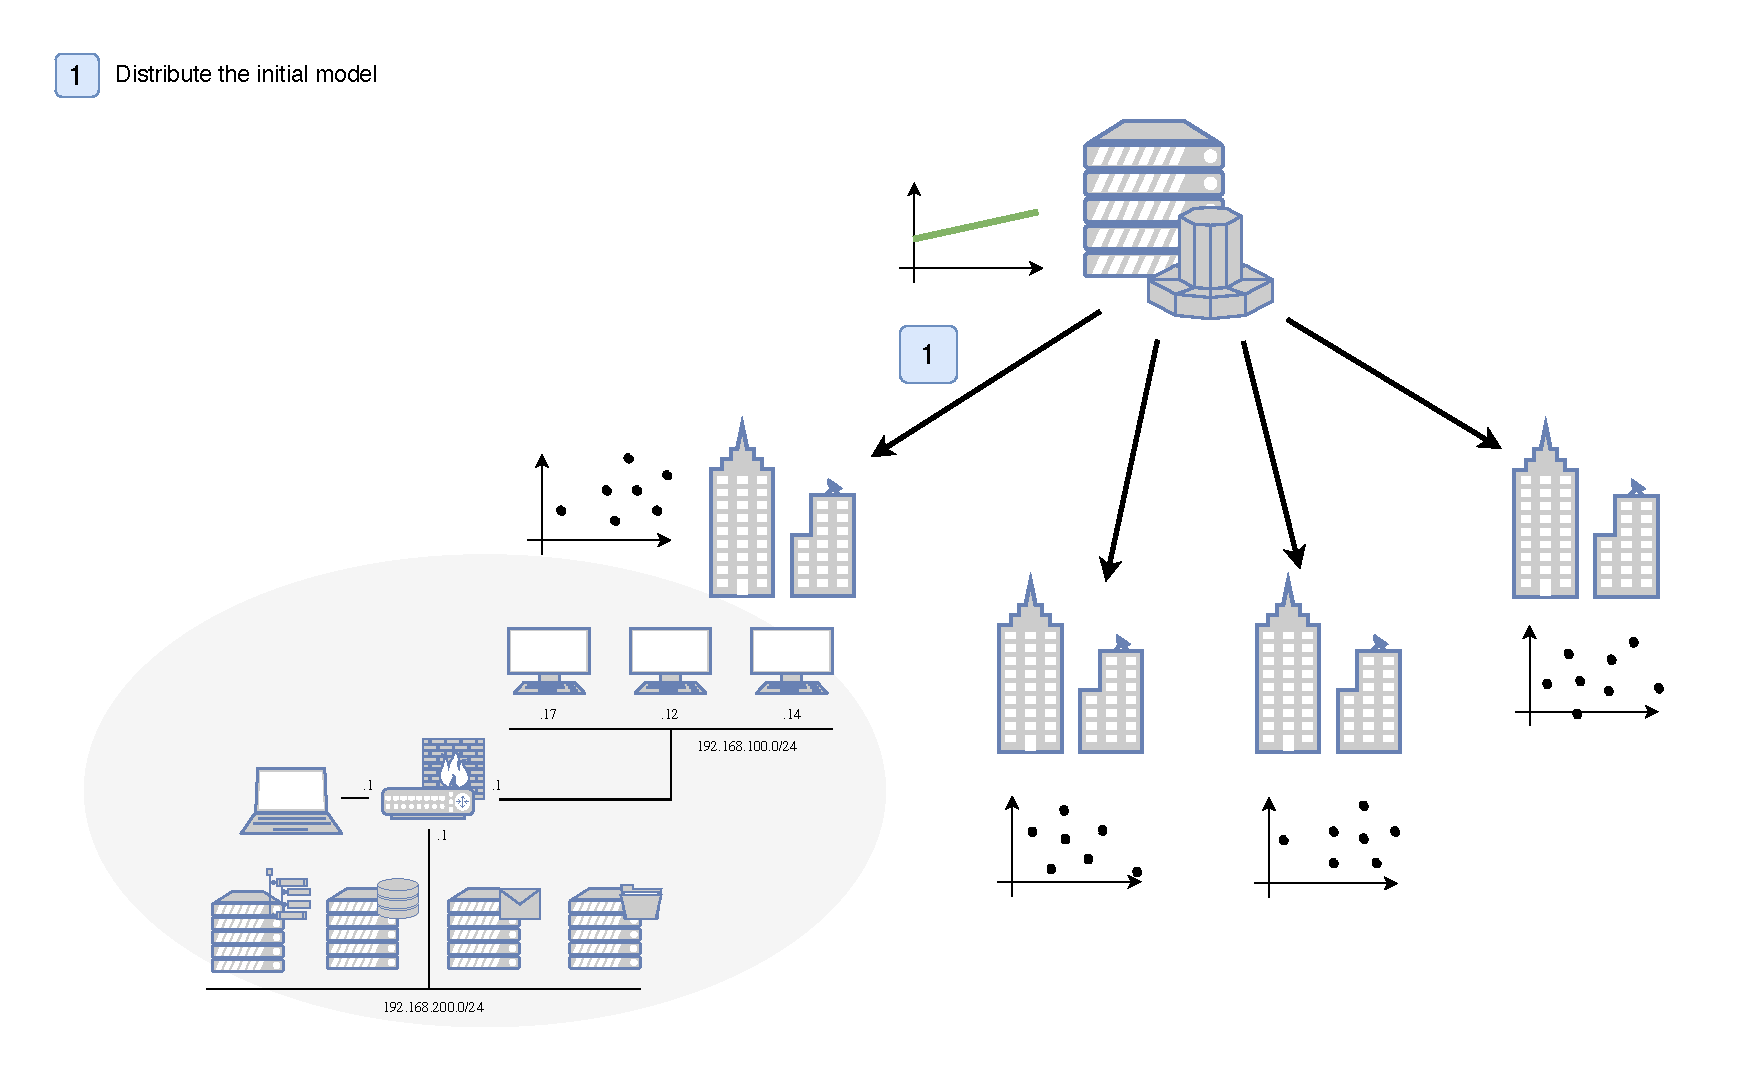
\includegraphics[width=.75\linewidth]{./figures/intro/fl/1.pdf}}%
    % Cannot use animations with MacOS Preview.
    % \only<3>{\animategraphics[width=.75\linewidth,loop,autoplay]{2}{./figures/intro/fl/2-}{1}{2}}%
    \only<3>{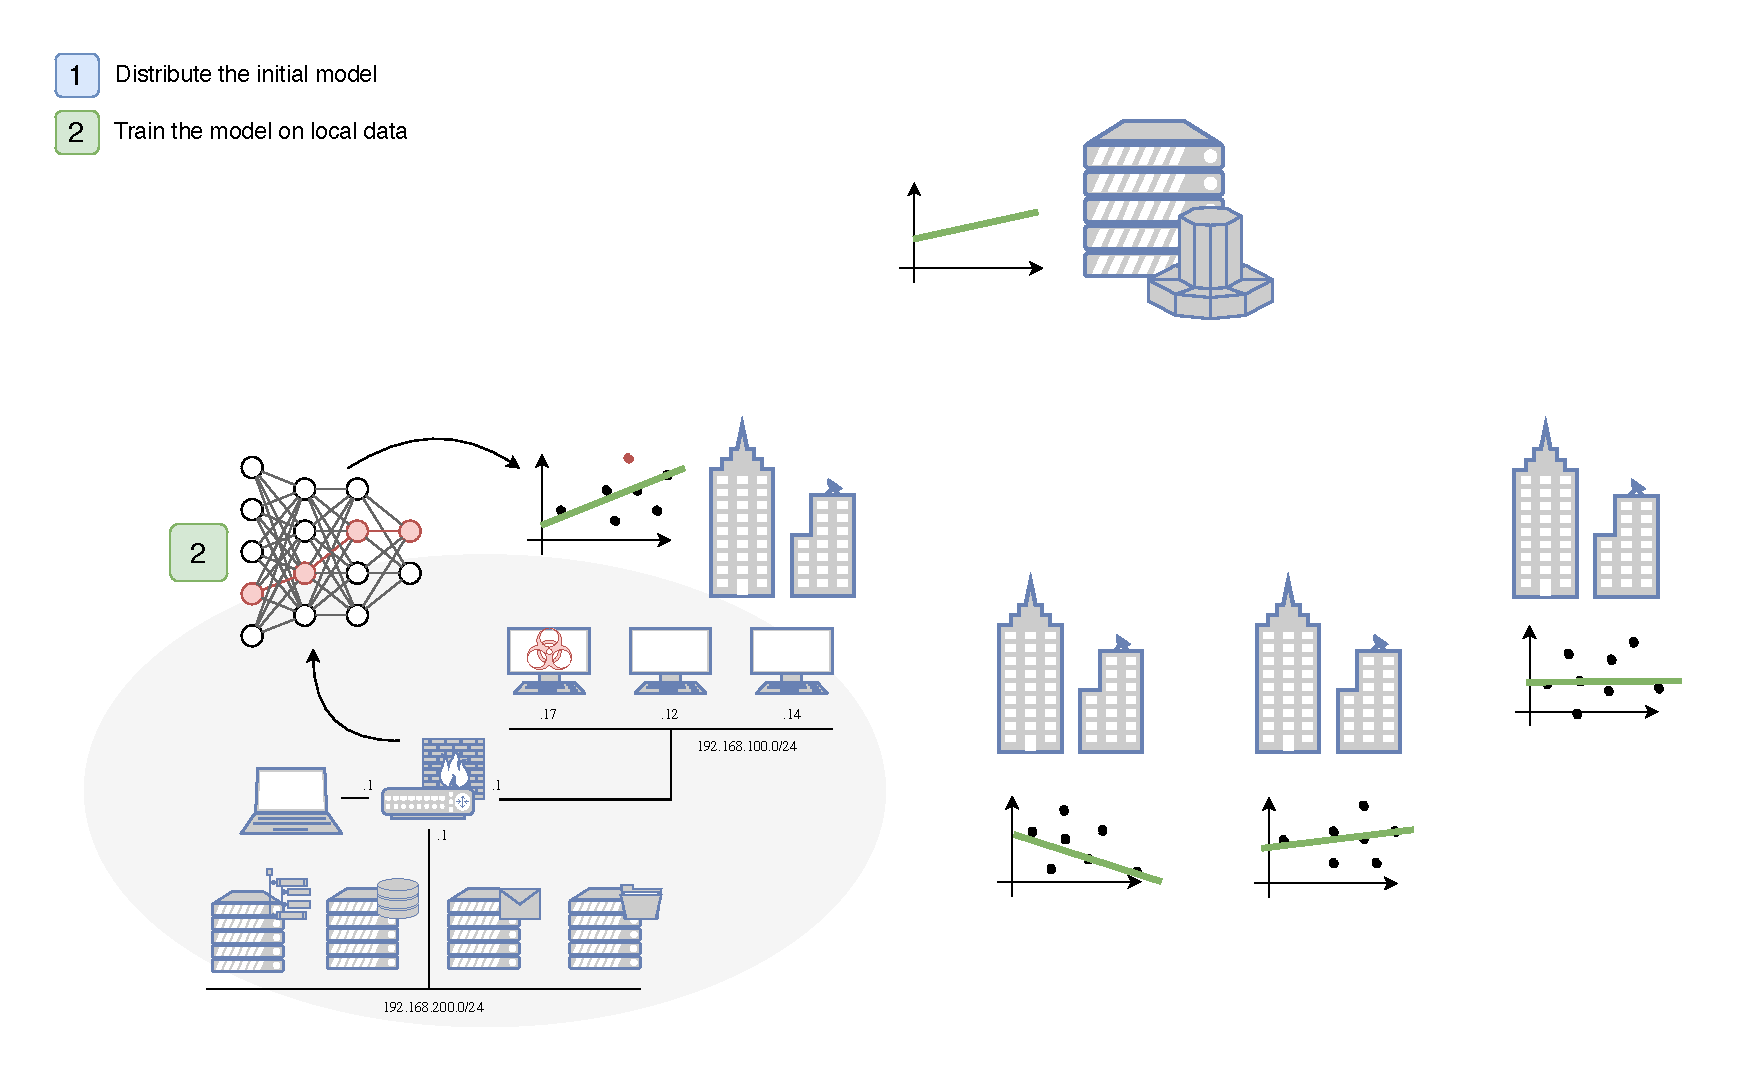
\includegraphics[width=.75\linewidth]{./figures/intro/fl/2-2.pdf}}%
    \only<4>{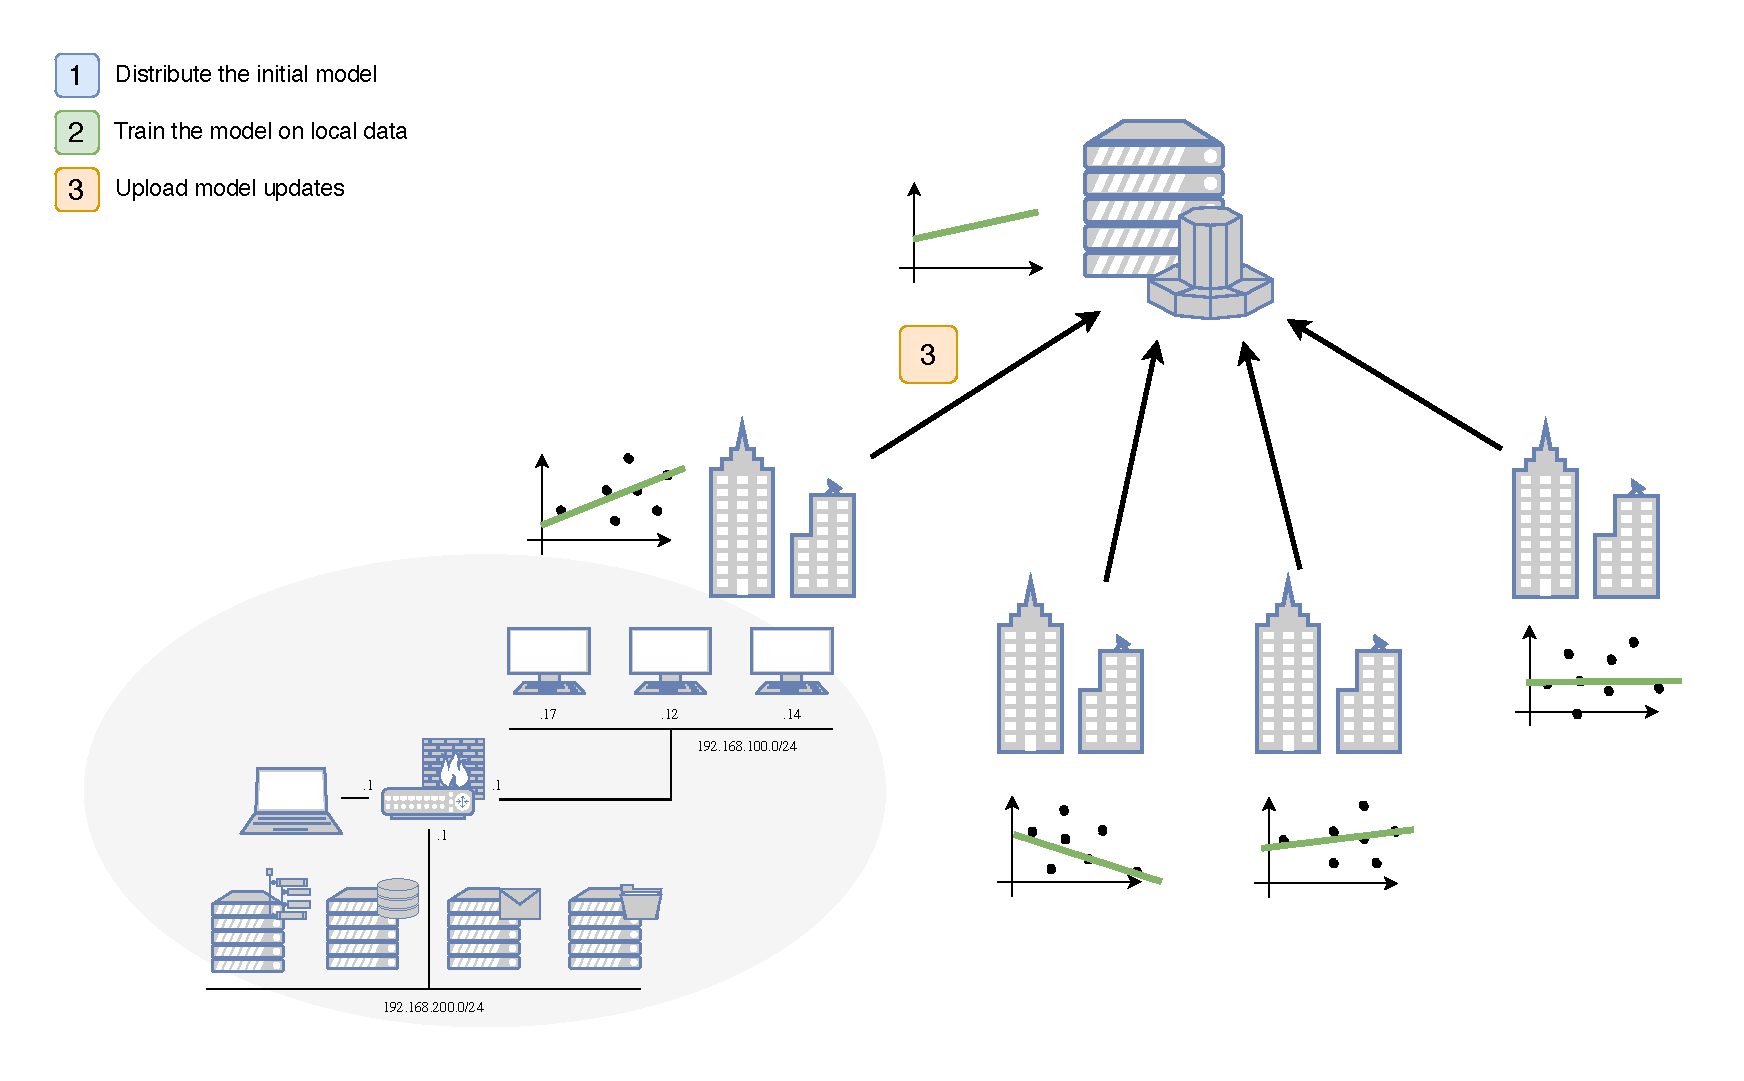
\includegraphics[width=.75\linewidth]{./figures/intro/fl/3.pdf}}%
    \only<5>{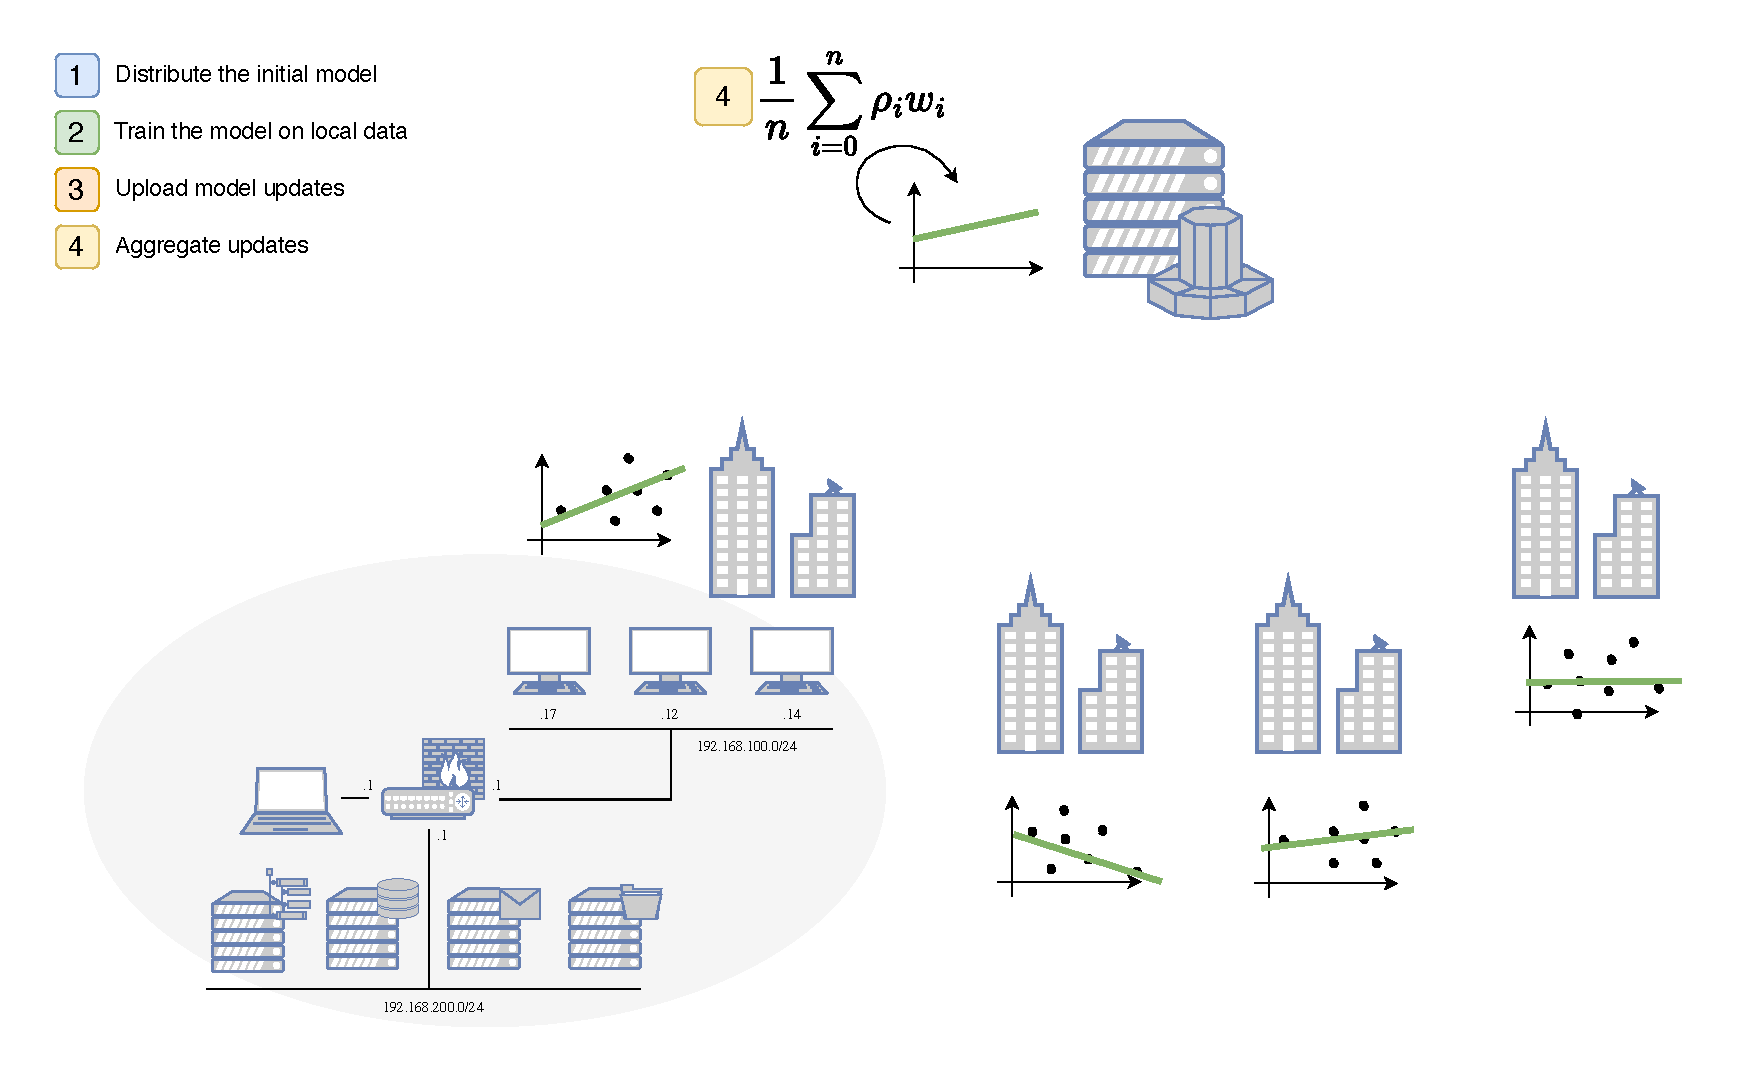
\includegraphics[width=.75\linewidth]{./figures/intro/fl/4.pdf}}%
    \only<6>{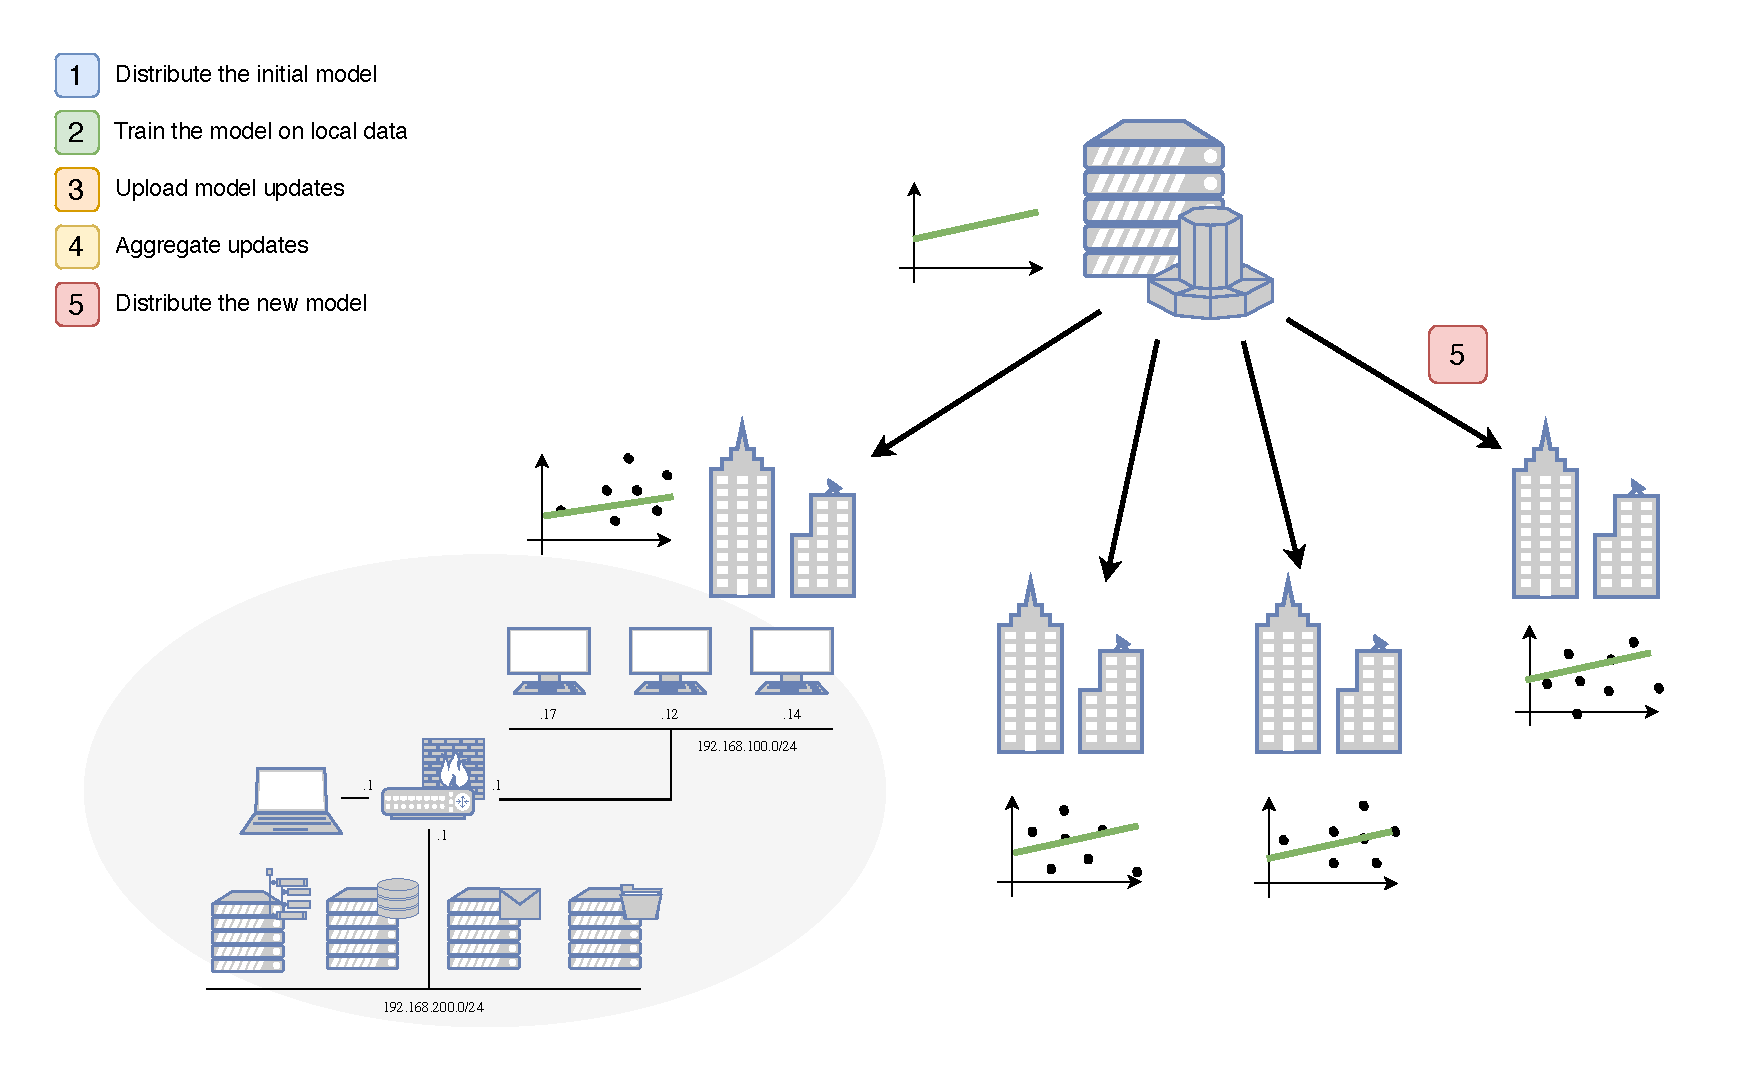
\includegraphics[width=.75\linewidth]{./figures/intro/fl/5.pdf}}%
    \only<7>{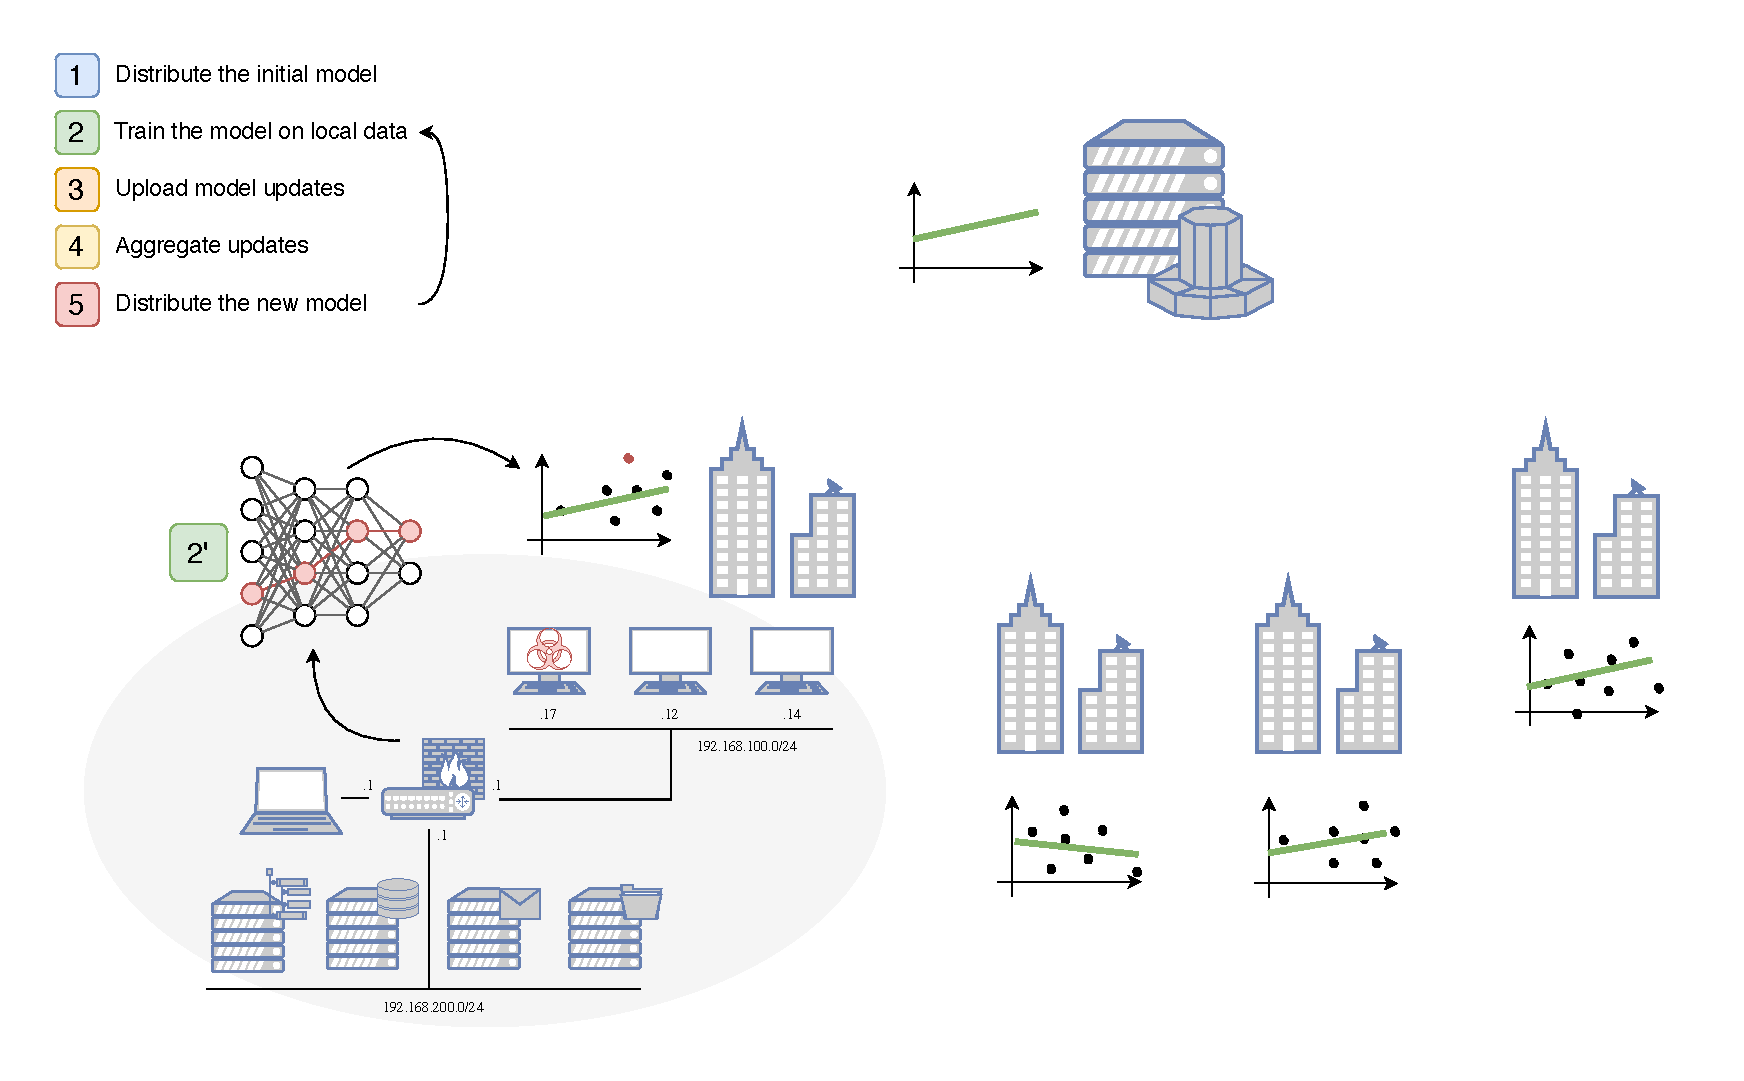
\includegraphics[width=.75\linewidth]{./figures/intro/fl/6.pdf}}%
    \caption{Typical FL workflow, applied to NIDSs.}
  \end{figure}
\end{frame}

\begin{frame}{FL for NIDSs}

  \textbf{Benefits}
  \begin{itemize}[<+->]
    \item Virtually extended dataset with Horizontal FL.
    \begin{itemize}[<1->]
      \item Better generalization.
      \item Reduced risk of overfitting or local bias.
    \end{itemize}
    

    \item Effectively share knowledge (\eg, on specific classes, instances) between participants
    \begin{itemize}[<1->]
      \item Share the knowledge about a new attack~\autocite{lavaur_icdcs_demo_2024};
      \item Improve the characterization of specific devices; \dots
    \end{itemize}

    \only<2>{\fcitefootnote{lavaur_icdcs_demo_2024}}

  \end{itemize}
\end{frame}